\documentclass{beamer}

\usepackage{inputenc}
\usepackage{graphicx}

\usetheme{Warsaw}

\title{Problem of Programming Language Concurrency Semantics}
\subtitle{Mark Batty, Kayvan Memarian, Kyndylan Nienhuis, Jean Pichon-Pharabod, Peter Sewell}   

\author{Presentation by \\ Akshay Gopalakrishnan}

\institute{McGill University}

\begin{document}
    
    %title page
    \begin{frame}

        \titlepage
    \end{frame}

    %Introduction
    \begin{frame}{Introduction/Goals}

        \begin{itemize}
            \item An overview of the current problems in semantically defining relaxed memory models.
            \item Give mechanized proof for DRF-SC property of C11 (HOL4).
            \item Thin air executions in C11 and its lack of understanding.
            \item Proof that per-candidate execution model of C11 cannot disallow thin air executions. 
            \item Operational model disallowing thin air behaviors but restricting compiler optimizations. 
            \item Difficulty in defining the C11 notion of undefined behavior.
        \end{itemize}
        

    \end{frame}

    % Start with SC and some examples
    \begin{frame}{Sequential Consistency - Examples}
        
        Simplest model of reasoning. 
        Interleaving semantics. 
        Informally,
        \center A concurrent program's outcome is equivalent to the same program being run in a uni-processor environment. 

        \textbf{Note}: Hardware exhibits Non-SC behaviors that give us better performance. 

    \end{frame}


    %Take previous examples and show that hardware exhibit relaxed behaviors too (TSO/LB)
    \begin{frame}{Hardware Features - x86, ARM, POWER}
        
        Store Buffering
        \begin{figure}
            \centering
            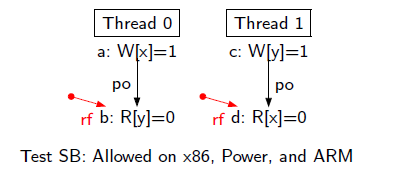
\includegraphics[scale=0.7]{SB.PNG}
        \end{figure}
        
    \end{frame}

    \begin{frame}{Hardware Features - x86, ARM, POWER}
        
        Message Passing
        \begin{figure}
            \centering
            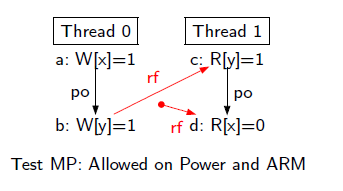
\includegraphics[scale=0.7]{MP.PNG}
        \end{figure}
        
    \end{frame}

    \begin{frame}{Hardware Features - x86, ARM, POWER}

        Non-Multi-Copy Atomicity
        \begin{figure}
            \centering
            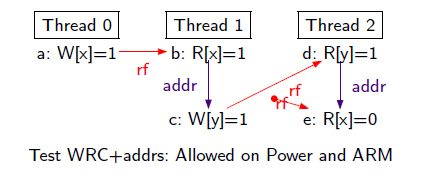
\includegraphics[scale=0.7]{WRC.PNG}
        \end{figure}

    \end{frame}

    %Introduction to data races
    \begin{frame}{Data Races}
        
        Such relaxed behaviors can give rise to what is known as Data Race.

        Consider timelines of two events operating on the same memory.
        \\
        -------------------------A
        \\
        ----------B

        Behaviors beyond A-then-B or B-then-A will be present in Non-SC executions.
        Now difficult to reason with programs. 
        
    \end{frame}

    \begin{frame}{DRF-SC model}
        Statement:
        \center If a program exhibits \textbf{no} data race in its SC executions, then it is guaranteed to have \textbf{only} SC behaviors.

        %Cite Adve and Gharchorloo
        Useful property for models of High Level Languages. 
        Is central to the C11 memory model. 
    \end{frame}

    %Overview of C11 and Java memory models
    \begin{frame}{High Level Language models - C11}
        
        \begin{itemize}
            \item Axiomatic model.
            \item Per-execution semantics.
            \item Description of disallowed behaviors using partial orders between program events in an execution.
            \item Has multiple degrees of atomicity - $RLX \ \geq \ REL \ \geq \ ACQ \ \geq \ CON \ \geq \ SC$.
            \item Has various partial order definitions between program events - $rf$, $sb$, $hb$, $mo$. 
            \item Exhibits DRF-SC property for programs not using low-level atomics (only $SC$).
        \end{itemize}
        
    \end{frame}

    %Overview of proof (state theorem) of DRF-SC for C11 memory model
    \begin{frame}{DRF-SC proof Theorem for C11 memory model}

        \begin{figure}
            \centering
            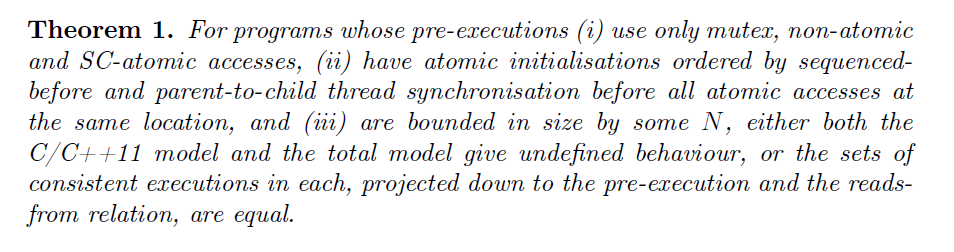
\includegraphics[scale=0.5]{DRF-SC.PNG}
        \end{figure}

        The total model captures only the SC semantics of the C11 memory model. 
        "Total" here being it is defined using only one total order between all events.
        
    \end{frame}

    \begin{frame}{Part 1}

        \centering For every consistent execution in the C11 model, there exists a consistent execution in the Total model with the same reads-from relation. 

        \centering For every consistent execution in the Total model, there exists a consistent execution in the C11 model with the same reads-from relation.
    \end{frame}

    \begin{frame}{Part 2}

        \centering For every racy execution in the C11 model, there exists a racy execution in the total model.

        The read values may not be the same, as the below example shows.
        \begin{figure}
            \centering
            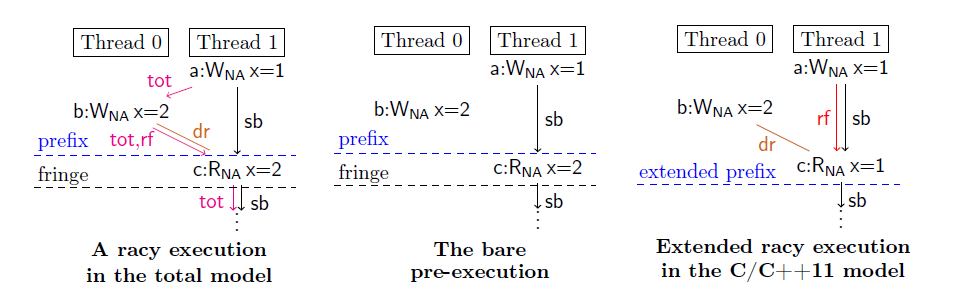
\includegraphics[scale=0.5]{RACY.PNG}
        \end{figure}

        Note: It is okay to have another racy execution with different read values as program exhibits undefined behavior anyways. 

    \end{frame}

    %Intro to OOTA using some examples from C11
    \begin{frame}{Thin Air problem (also known as Out-of-thin-air(OOTA))}
        
        Even though we restrict data-races in a program, semantically it is difficult to avoid certain outcomes that must be forbidden. 
        For instance, the following outcome should be disallowed:

        \begin{figure}
            \centering
            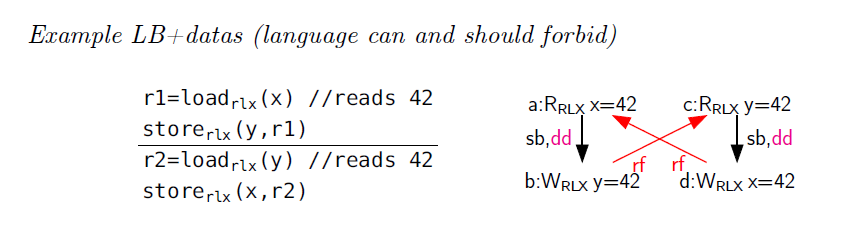
\includegraphics[scale=0.5]{LB+DD.PNG}
        \end{figure}
        
    \end{frame}

    \begin{frame}{OOTA cnt'd}
        
        But disallowing the previous execution, will also disallow the following load buffering (load-store reordering) case:
        \begin{figure}
            \centering
            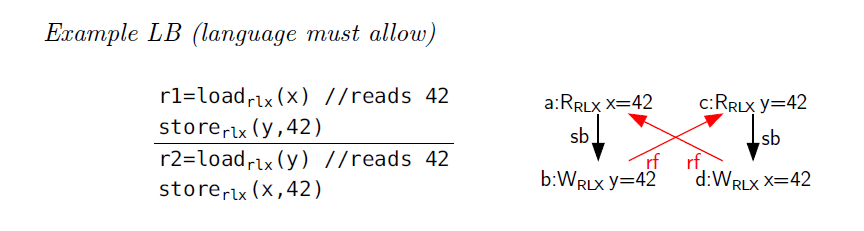
\includegraphics[scale=0.5]{LB.PNG}
        \end{figure}

    \end{frame}

    \begin{frame}{OOTA cnt'd}

        Some variants, after transformations, the outcomes should be allowed.

        %\begin{columns}
            
        %    \begin{column}[l]{5cm}
                \begin{figure}
                    \centering
                    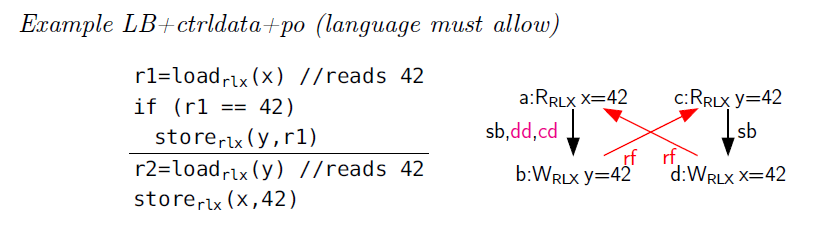
\includegraphics[scale=0.5]{LB+Ctrl+data.PNG}
                \end{figure}
        %    \end{column}

        %    \begin{column}[r]{5cm}
                \begin{figure}
                    \centering
                    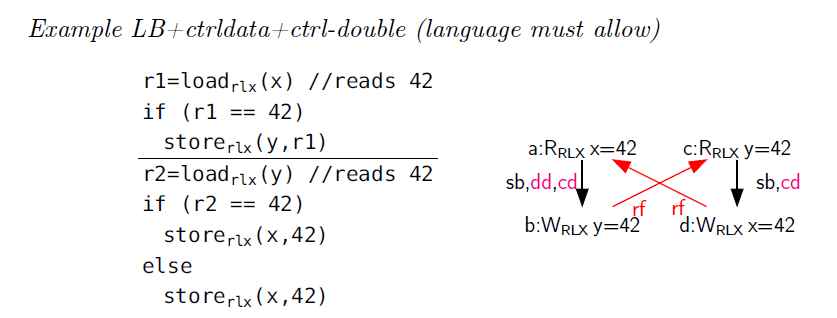
\includegraphics[scale=0.5]{LB+Ctrldata+ctrldouble.PNG}
                \end{figure}
        %    \end{column}

        %\end{columns}
        
    \end{frame}

    %Start with the example given in paper and display its variants. 
    \begin{frame}{Difficulty in semantically defining OOTA using per-candidate execution model}
        
        The above variants of programs have the exact candidate execution pattern in C11 style semantics.
        Hence, the possibility of semantically disallowing OOTA using this style is not possible. 
        
        \begin{figure}
            \centering
            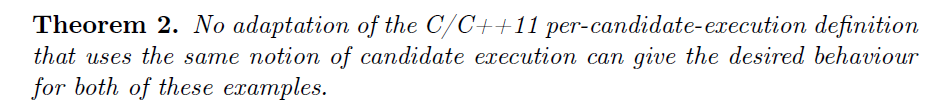
\includegraphics[scale=0.6]{OOTA-Thm.PNG}
        \end{figure}

    \end{frame}

    %Summarize other work done in preventing OOTA in C11
    \begin{frame}{Alterative solution - Operational model}
        %A figure explaining the definition of LTS, frontier, and extended frontier
        A labelled transition system for each thread, depicting thread-local semantics.
        Has all possible reachable states. 

        \begin{figure}
            \centering
            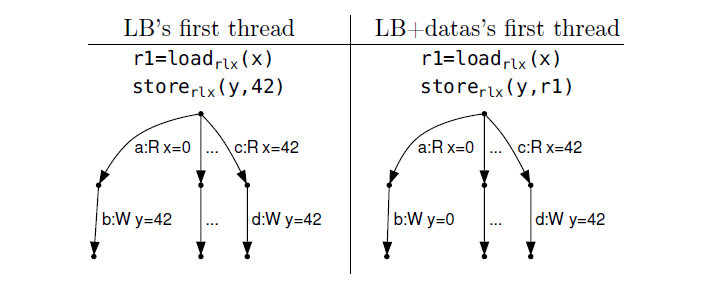
\includegraphics[scale=0.7]{Out-of-order-Oper.PNG}
        \end{figure}

    \end{frame}

    \begin{frame}{Operational model - cnt'd}
        
        States are LTS in-order with some edges \textit{ticked}.
        A set of edges can be "ticked" iff:
        \begin{itemize}
            \item Set of edges is non-empty.
            \item The edges themselves are not ticked.
            \item Edges have the same memory action label.
            \item Each non-discarded path is either having its event in the set being ticked, or the path discarded due to tick.
            \item No edge is blocked (due to control dependency for example).
        \end{itemize}
        
        \center The above semantics would cover all our previous examples of LB and its variants. 
    \end{frame}

    %Addresses our OOTA examples
    \begin{frame}{Problem of Compiler Optimizations}
        %Still unsure how it addresses completely, need to look back at it once again. 
        Irrelevant read elimination:
        \begin{figure}
            \centering
            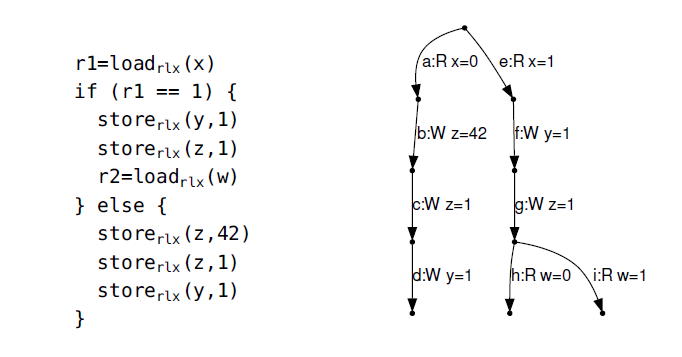
\includegraphics[scale=0.7]{IRR-RD.PNG}
        \end{figure}
    \end{frame}

    %Impact on compiler optimizations
    \begin{frame}{Problem of Compiler optimizations - cnt'd}
        Inter-thread optimizations
        \begin{figure}
            \centering
            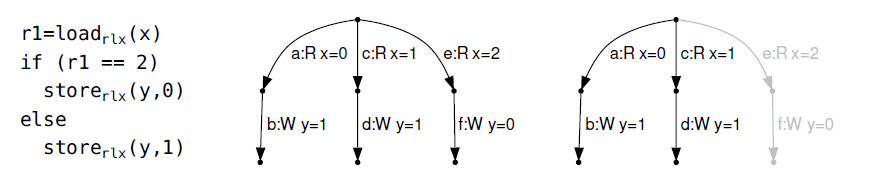
\includegraphics[scale=0.7]{INTER-THREAD-OPT.PNG}
        \end{figure}
        %Need for recursive definition but how vast would it be?
    \end{frame}

    %Notion of undefined behavior in C11
    \begin{frame}{"Undefined" in C/C11}

        Undefined literally gives no semantics for the programs in C11.

        Examples of programs that would exhibit undefined behavior are:
        \begin{itemize}
            \item Out of bounds array accesses.
            \item Divide by zero.
            \item Programs with data races.
        \end{itemize}

        %Examples for asserting undefined behavior - Out-of-bounds Array access, Divide-by-zero, Data-race
        
    \end{frame}

    %Example using Divide-by-zero
    \begin{frame}{Example asserting Divide-by-zero}
        %A weird example indeed, but can do it because of undefined behavior. 
        
        \begin{figure}
            \centering
            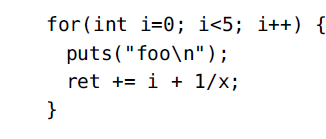
\includegraphics[scale=0.7]{DIV-ZERO.PNG}
        \end{figure}

        Loop invariant code motion is possible, due to $x$ being zero.
        Thus, the compiler is free to move $1/x$ outside the loop itself, as a form of optimization.

    \end{frame}

    %Example of Concurrent program asserting OOBA case
    \begin{frame}{Example asserting OOBA in a concurrent program}
        %Another weird example.
        \begin{figure}
            \centering
            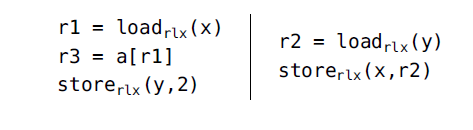
\includegraphics[scale=0.7]{OOBA+RLX.PNG}
        \end{figure}

        SC semantics would not give OOBA. //
        But C11 semantics pertaining ARM/POWER H/W would ensure OOBA (through means of Load Buffering), thus undefined behavior.
    \end{frame}

    %Conclusion slide
    \begin{frame}{Conclusion}
        \begin{enumerate}
            \item Hardware exhibits relaxed memory behaviors for better performance. 
            \item C11 semantics inevitably allows thin-air executions.
            \item No per-candidate C11 execution style can capture thin-air execution semantics. 
            \item An operational model to remedy it inevitably asks for taking into account of all possible compiler optimizations. 
            \item Lack of semantics for C11 Undefined behavior makes it difficult to reason about programs and impact on it due to compiler optimizations. 
        \end{enumerate}
    \end{frame}

    \begin{frame}{Thank you}

        Questions?
        
    \end{frame}

\end{document}